% Copyright 2009 James Hensman and Michael Dewar
% Licensed under the Gnu General Public license, see COPYING
\documentclass{article}
\title{pyvb: Variational Bayesian Networks in python}
\author{James Hensman, Mike Dewar}
\date{\today}


\usepackage{amsmath}
\usepackage{amsfonts}
\usepackage{graphicx}
\usepackage{natbib}

\setlength{\textwidth}{16cm}
\setlength{\oddsidemargin}{0cm}
\setlength{\evensidemargin}{0cm}

\newcommand{\const}{\textit{const.}}
\newcommand{\tr}{\textit{tr}}
\newcommand{\qs}{q^\star}
\newcommand{\<}{\langle}
\renewcommand{\>}{\rangle}
\newcommand{\trace}{\textit{tr}}
\begin{document}
\maketitle

\section{Bayesian Networks}

\section{Variational Bayes}
Some directed probabilistic models cannot be solved in closed form. A common approach is to use a Markov Chain Monte Carlo (MCMC) sampling method, (see for example the excellent {\em pymc} project \cite{pymc}).  In the limit of an infinite number of samples, the MCMC method provides perfect inference of the posterior probability density (see any statistics textbook for a proof), and a high number of samples provides an {\em approximation} to the posterior.  

Similarly in Variational Bayes, an approximation to the posterior is made by way of some {\em factorial} distribution $q$:
\begin{equation}
p(A,B,\ldots) \approx q_A(A) q_B(B) \ldots
\end{equation}

For convenience, $q_A(A)$ is often written as $q(A)$, $q_B(B)$ as $q(B)$ et cetera, since the function can be determined by its argument. 

The distribution $q$ is `optimised' by finding the distribution $q$ which minimises the KL divergence between $p(A,B,\ldots)$ and $q(A,B,\ldots)$.  After some long and arduous mathematics, \citet{Bishop2006prm} yeilds

\begin{equation}
\ln \qs(A) = \< \ln p(A,B,\ldots)\>_{q(\bar A)}
\label{eq:VB_update}
\end{equation}

That is, the distribution $\qs(A)$ which minimises the KL divergence between $q$ and $p$ can be found by taking the expected value of the joint-log-probability, under the current ($q$) distribution of all other unknown variables. 

\section{Markov blankets}
In a directed Bayesian network, a node $A$ is dependent only upon its {\em Markov Blanket}: that is its parents, children, and children's parents. Formally, one can write
\begin{equation}
p(A|\partial A,B) = p(A | \partial A)
\end{equation}
where $\partial A$ is the Markov blanket of A and B is the set of all other variables.   

This has important consequenses when coding a set of nodes to do implement the VB algorithm: each node must be `aware' of nodes in his Markov Blanket. Additionall, he must be aware of his {\em relationship} with said nodes. In pyvb, each node instance contains pointers to its parents, as well as a list of child nodes.  Co-parents (child nodes' other parents) are dealt with either by messages passed from the child nodes, or by {\em operation} nodes, which define how two parent nodes combine to become the parent of a common child (such as by addition).  

\section{Network Structure in pyvb}
In pyvb, all random variables are represented by an instance of an appropriate class. There are classes for Gaussian nodes, Gamma nodes and Wishart nodes. More random variables are to be implemented in future (see TODO).

Additionally, {\em operations} are represented by instances of classes. There are classes to represent addition, multiplication and horizontal stacking (hstack).  This provides an easy way to deal with co-parents: when a node seeks messages in order to update, the operation nodes automatically account for a co-parent. Some of the code in the operation classes is a little complicated: this is where messages are `modified' according to the operation.  This document seeks to explain the workings of these nodes.   

The basic node class, from which Gaussian nodes inherrit, is capable of operations such as addition amd multiplication. This means that one can instantiate a pair of nodes, and then add them using the `+' operator: this creates and returns an instance of the Addition class, with the two original nodes as parents. 

Each node then has two `parents': in a Gaussian node the `mean\_parent' and `precision\_parent' attributes are pointers to the apppropriate nodes; in an Addition node the attributes `A' and `B' are pointers to the two nodes to be added; in the Gamma node the attributes `a0' and `b0' are pointers to the appropriate nodes and so on.

We have bastardised the standard nomenclature slightly: strictly a node can have more than two `true' parents. In our implementation, operation nodes are used to facilitate this. For example, the graphical model of Figure \ref{fig:gm_true_bastard}(a) represents a Gaussian node $C$ and its three parents $A$,$B$ and $\Lambda_C$.  The diagram in Figure \ref{fig:gm_true_bastard}(b) shows how an operation node (in this case addition) can be used to represent this. 

\begin{figure}
\centering
\begin{minipage}{0.4\textwidth}
\begin{center}
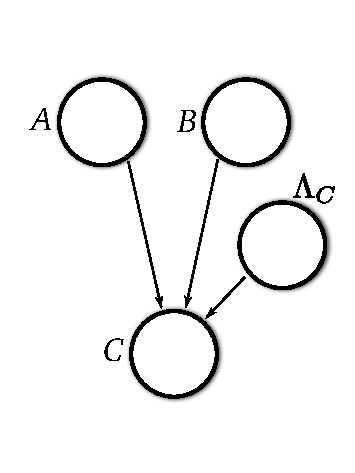
\includegraphics[width=\textwidth]{images/gm_true}
(a)
\end{center}
\end{minipage}
\begin{minipage}{0.4\textwidth}
\begin{center}
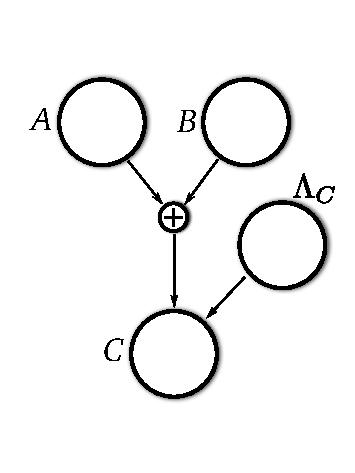
\includegraphics[width=\textwidth]{images/gm_bastard}
(b)
\end{center}
\end{minipage}
\caption{(a) A simple Graphical model.  (b) A diagram showing the introduction of an operation node.}
\label{fig:gm_true_bastard}
\end{figure}


Each node can have an arbitrary number of children: again, children can be either Gaussian nodes or operation nodes. 

{\bf Note}: The node instances are not `aware' of the nature of the nodes around them in the network. They simply expect to be passed appropriate messages when updating. 


\section{A Gaussian Node}
Consider the simple DAG in Figure \ref{fig:simple_DAG}.  $A$ is the `mean\_parent' of $B$, and $\Lambda_B$ is the `precision\_parent' of $B$. That, is, one can write the joint probability of the nodes as
\begin{equation}
\begin{split}
p(A,B,\Lambda_B) &= p(A) p(B | A, \Lambda_B) p(\Lambda_B)\\
&= \mathcal N (A|\mu_A, \Lambda_A) \mathcal N (B | A, \Lambda_B) \mathcal {Ga}(\Lambda_B | \nu_0, W_0)
\end{split}
\end{equation}
assuming that the priors on $A$ and $\Lambda_B$ have fixed parameters: hopefully the notation is obvious.  

\begin{figure}
\centering
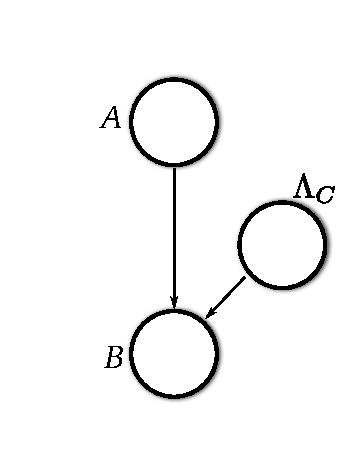
\includegraphics{images/simple_DAG}
\caption{A simple network with two Gausian nodes.}
\label{fig:simple_DAG}
\end{figure}

It is trivial to write out the log of the joint probability: for convenience, we write it as $-2 \ln p(.)$:
\begin{equation}
-2 \ln p(A,B,\Lambda_B) = (A-\mu_A)^\top\lambda_A(A-\mu_A) + (B-A)^\top\Lambda_B(B-A) + \tr (W_0^{-1}\Lambda_B) + \ln|\Lambda_B| + \const
\end{equation}
where we have followed \cite{Bishop2006prm} in incorporating irrelevant terms into {\em const}.  

\subsection{Updating the node}
We are now ready to apply the variational updates to the node A. Recalling (\ref{eq:VB_update}):
\begin{equation}
\begin{split}
-2 \ln \qs (A) &= \big< A^\top\lambda_A A -2A^\top\Lambda_A\mu_A + A^\top\Lambda_B A  - 2A^\top \Lambda_B B \big> + \const\\
 &= A^\top(\Lambda_A + \<\Lambda_B\>)A -2A^\top(\Lambda_A\mu_A + \<\Lambda_B\> \<B\>) + \const
\end{split}
\end{equation}
This can be recognised as the log of a Gaussian with precision $\Lambda_A + \<\Lambda_B\>$ and mean $(\Lambda_A + \<\Lambda_B\>)^{-1}(\Lambda_A\mu_A + \<\Lambda_B\> \<B\>)$. 

Within the pyvb code, the $\<\Lambda_B\>$ `message' is known as `m1', and the $\<\Lambda_B\> \<B\>$ message is known as m2: these are the messages which flow `up' the arrows. 

In pyvb, this is implemented as follows:
\begin{enumerate}
\item Each node has a method `pass\_down\_Ex', where is returns its expected value. 
\item Each {\em Gaussian} node has a method `pass\_up\_m1_m2', which fetches the expected value of its precision parent and returns it, along with the matrix multiplication of this value and the node's own expected value (or {\em mean})\footnote{It may seem easier for Gaussian node to pass up its precision and expected value separately: the adopted convention makes life easier when dealing with operations, as we shall see}. 
\item Each Gaussian node has a method called `update', which requests the above messages from parent and child nodes, and applies the suitable linear algebra.
\end{enumerate}

\subsection{Multiple Children}
If the node $A$ were to have multiple (Gaussian) children, all we need to do is to {\em add up} the messages. So when a node with multiple children needs to update, it simple requests the messages m1 and m2 from each of the children, adds them up and proceeds as before.  

TODO: demonstration/proof.  



\section{Operations}
\subsection{Addition}
\subsection{Multiplication}
\subsubsection{Left Multiplier}
Consider the updating of a node $A$, with parent nodes $\mu_A$ and $\Lambda_A$.  $A$ has a child node $C$, with co-parents $\Lambda_C$ and (through multipication) $B$.  The situation is shown in Figure \ref{fig:mult_markov}:
note that the nodes $B$,$C$,$\mu_A$ and $\Lambda_A$ form the Markov blanket of A, and so no other information is required for the update - even if the network stretched for many nodes in any direction.  

We're assuming the $A$ is right-multiplied by $B$, i.e. we have $p(C) = \mathcal{N}(C | AB, \Lambda_C)$.  The log joint probability is:
	
\begin{equation}
%-2 \log p(.) = -2\ln p(A) -2\ln p(B) + (C-AB)^\top\Lambda_C(C-AB)\\ 
-2 \log p(.) = -2\ln p(A) -2\ln p(B) + C^\top\Lambda_CC + B^\top A^\top \Lambda_C AB -2 C^\top \Lambda_C AB + \const
\end{equation}.  

Applying the update rule (\ref{eq:VB_update}), we obtain
\begin{equation}
-2\ln \qs(A) = -2 \ln p(A) + \< B^\top A^\top \Lambda_C AB -2 C^\top \Lambda_C AB \> + \const
\label{eq:mult1}
\end{equation}
which, as might be expected, is quadratic in A, making $\qs(A)$ a Gaussian. The messages passed to the node $A$ depend on the orientation of $A$ and $B$:
\begin{enumerate}
\item $B$ is scalar (meaning $A$ must be a vector to match the size of$\Lambda_C$): m1 becomes $\<\Lambda_C\>\<BB^\top\>$, m2 becomes $\<\Lambda_C\>\<C\>\<B\>$. Since the m1 message received from $C$ is $\<\Lambda_C\>\<C\>$, all that has to be done is to multiply this by $\<B\>$ (which is scalar).
\item $B$ is a vector, and $A$ is a transposed vector. In this case, $\<C\>$ and $\<\Lambda_C\>$ must be scalar, rendering the order of multiplication unimportant: the messages passed are $\<\Lambda_C\>\<BB^\top\>$ and $\<B\>\<\Lambda_C\>\<C\>$, which is $\<B\>$ times the message m2 from the node $C$.  
\item $B$ is a vector, and $A$ is a matrix.  In this case, the addition node passes up m1 from $C$ and $\<BB^\top\>$ (which is a matrix) for the hstack node above to deal with (see \ref{hstack}).  
\end{enumerate}


\subsubsection{Right Multiplier}
In pyvb, the node on the right hand side of any multiplication is constrained to being a vector - either a Gaussian or Constant instance.  
Consider the same situation as above but for the updating of node $B$.  Figure {??} shows $B$'s Markov blanket. The joint double negative probability is written as:
\begin{equation}
-2\ln p(.) = -2\ln p(A) + (B-\mu_B)^\top\Lambda_B(B-\mu_B) + (C-AB)^\top\Lambda_C(C-AB)+\const
\end{equation}
multiplying out the brackets and appliying (\ref{eq:VB_update}) yeilds
\begin{equation}
\begin{split}
-2\ln \qs (B) &= \big< B^\top\Lambda_BB -2B^\top\Lambda_B\mu_B +  B^\top A^\top \Lambda_C AB -2 C^\top \Lambda_C AB \big>+ \const\\
& = B^\top(\<\Lambda_B\> + \<A^\top \Lambda_C A\>)B -2B^\top(\<\Lambda_B\>\<\mu_B\> +\<A^\top\> \<\Lambda_C\>\<C\>) + \const
\end{split}
\end{equation}

As is to be expected, the format implies that $\qs(B)$ is Gaussian.  The message m2 is simple: the multiplication node simply needs to fetch the m2 message from $C$ and multiply by $\<A\>$ before returning it to B.  The m1 message is more copmlicated in this case, and some care needs to be taken:
\begin{enumerate}
\item $C$ is scalar: the order of multiplication becomes unimportant and the m1 message is simply $\<A^\top A\>\<\Lambda_C\>$.
\item $A$ is a constant matrix: m1 becomes simply $A^\top \<\Lambda_C\>A$.  
\item $A$ is a hstacked matrix (see \ref{hstack}). The message m1 becomes a matrix with element $[i,j]$ equal to $\trace(\<A_iA_j^\top\>\<\Lambda_C\>)$, where $A_i$ is the $i^{th}$ column of $A$.    
\end{enumerate}

\subsubsection{Child of Multiples}
The updating of the final node $C$ is simpler than that for its parents. One only requires to know the expected value of $AB$, which is trivial.


\begin{figure}
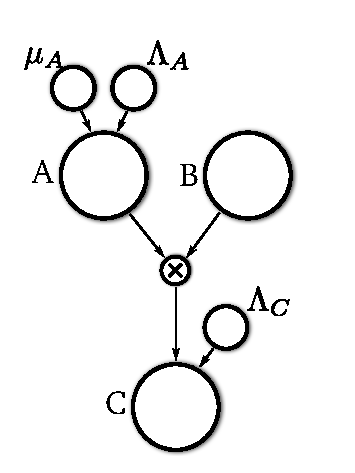
\includegraphics{images/mult_markov}
\caption{The markov blanket of the node A}
\label{fig:mult_markov}
\end{figure}

\subsection{Hstacking}
\label{hstack}
Sometimes (often!) it is necessary to involve a matrix operation in our model.  For example, in a Linear Dynamic System, the update to the state is given by multiplying the old state by the state transition matrix $A$ (see \ref{examples:LDS}).  The matrix in question is not nessesarily square, nor non-negative definite. It turns out that an appropriate (and conjugate!) prior of such a matrix is Gaussian. For convenience, we offer the {\em hstack} node, which allows one to create a random matrix with Gaussian priors over the columns.  

\subsubsection{Adding Hstacks}
This is not supported yet, don't try it!

\subsubsection{Mutiplying Hstacks}
Recall the multiplication case of section \ref{multiplication}.  Where the prior over $A$ is a series of Gaussians over the columns of $A$ (which we shall denote $A_i$), equation (\ref{eq:mult1}) becomes
\begin{equation}
\begin{split}
-2\ln \qs(A) &= \bigg<\sum_i \big\{(A_i-\mu_{Ai})^\top \Lambda_{Ai}(A_i-\mu_{Ai})\big\}\bigg> + \< B^\top A^\top \Lambda_C AB -2 C^\top \Lambda_C AB \> + \const\\
&= \sum_i \big\{ A_i^\top \<\Lambda_{Ai}\> A_i -2 A_i^\top\<\Lambda_{Ai}\>\<\mu_{Ai}\> \big\}  + \sum_i \sum_j \big\{A_i^\top \<\Lambda_C\> A_j \<BB^\top\>_{[i,j]} \big\} -2 \sum_i \<C\>\<\Lambda_C\>A_i \<B\>_{[i]} + \const\\
&= \sum_i \Bigg\{ A_i^\top \bigg(\<\Lambda_{Ai}\> +  \<\Lambda_C\>  \<BB^\top\>_{[i,i]}\bigg) A_i -2 A_i^\top\bigg(\<\Lambda_{Ai}\>\<\mu_{Ai}\>   - \sum_{j!=i} \big\{ \<\Lambda_C\> \<BB^\top\>_{[i,j]} A_j \big\}\\
& + \<C\>\<\Lambda_C\>A_i \<B\>_{[i]} \bigg)\Bigg\} + \const
\end{split}
\label{eq:hstack1}
\end{equation}
The subscript with square brackets represents an index, i.e. $\<B\>_{[i]}$ is the $i^{th}$ element of the vector $\<B\>$, and $\<BB^\top\>_{[i,i]}$ is the $i,j^{th}$ element of the matrix $\<BB^\top\>$. 

Since (\ref{eq:hstack1}) is a summation of quadratics, the $q$ distributions of $A_i$ must be independent Gaussians.  The m1 and m2 messages to be passed from the hstack node to a single Gaussian column $A_i$ are:
\begin{equation}
\begin{split}
m1 &=  \<\Lambda_C\>  \<BB^\top\>_{[i,i]}\\
m2 &=   \<C\>\<\Lambda_C\>\<B\>_{[i]}  - \sum_{j!=i} \big\{ \<\Lambda_C\> \<BB^\top\>_{[i,j]} \<A_j\> \big\}  
\end{split}
\end{equation}

\section{Precision Nodes}
\section{Gamma}
\section{Diagonal Gamma}
\section{Wishart}

\section{Examples}
\subsection{Linear Regression}
\subsection{Principal Component Analysis}

\subsection{Linear Dynamic System}
\label{examples:LDS}
In the KF, we do
\begin{equation}
p(x_t) = \int p(x_t | x_{t-1}) p(x_t | y_t) p(x_{t-1}) d x_{t-1}
\end{equation}

In the variational equivalent, we do
\begin{equation}
\begin{split}
\ln q^\star(x_t) &= \int \ln \left( p(x_t | x_{t-1}) p(x_t | y_t) \right) q(x_{t-1}) d x_{t-1}\\
            &= \left<  \ln  p(x_t | x_{t-1})  + \ln p(x_t | y_t)  \right>_{q(x_{t-1})}
\end{split}
\end{equation}


\section{Appendix}
\subsection{The Gaussian Distribution}
\subsection{The Gamma Distribution}
\subsection{The Wishart Distribution}

\end{document}